%%%%%%%%%%%%%%%%%%%%%%%%%%%%%%%%%%%%%%%%%%%%%%%%%%%%%%%%
%%%%                                              %%%%%%
%%%%  Author: Peter Wilson                        %%%%%%
%%%%                                              %%%%%%
%%%%  ANDES quad element                          %%%%%%
%%%%                                              %%%%%%
%%%%%%%%%%%%%%%%%%%%%%%%%%%%%%%%%%%%%%%%%%%%%%%%%%%%%%%%


%fref generates automatically the respective abreviation/word in the text for the reference. You just have to define a label starting with the respective keyword.
%english: chap, sec, fig, eq, app
%deutsch: chap/kap, abs, abb, gl, anh
%see http://ctan.space-pro.be/tex-archive/macros/latex/contrib/fancyref/fancyref.pdf for more information



\setcounter{MaxMatrixCols}{20}
%\captionsetup{justification=centering}

\chapter[ANDES-DKQ quadrilateral shell element]{ANDES-DKQ quadrilateral \\ shell element}
\renewcommand{\Thema}{ANDES-DKT quadrilateral shell element}

The following chapter outlines the formulation and implementation of the stiffness matrix, mass matrix and quantity recovery for the ANDES-DKQ quadrilateral shell element in Kratos.

\section{Stiffness matrix formulation}

As per the element technology discussion in section \ref{FE_tech}, the ANDES-DKQ element uses different finite element technologies for the membrane and bending components, both of which are subsequently developed. 

\subsection{ANDES membrane formulation}

The membrane formulation is responsible for providing the membrane stiffness of the element. Unlike the linear triangle DSG element, bilinear quadrilaterals are susceptible to membrane locking, and, as such, the ANDES membrane formulation was prudentially chosen as presented in \cite{Hau94}. A full description and theoretical derivation of the ANDES approach falls outside the scope of this document, however, those interested are directed to Militello's and Felippa's initial paper \cite{Fel91} on the formulation.

Only the membrane portion of the total shell element is considered in this section, in which there are three DOFs per node.

\begin{equation} 
\mathbf{u}^T = 
\begin{pmatrix}
\mathbf{u}_1 & \mathbf{u}_2 & \mathbf{u}_3 & \mathbf{u}_4
\end{pmatrix} 
\hspace{10mm}
where
\hspace{10mm}
\mathbf{u}{_i}^T = 
\begin{pmatrix}
{u_{xi}} & {u_{yi}} & {\beta_{zi}}
\end{pmatrix}
\label{equation04}
\end{equation}

The ANDES membrane formulation, following the FF framework, is split into the basic stiffness related to the basic constant strain displacement matrix $\mathbf{L}$ and the higher order stiffness related to the higher order deviatoric strain displacement matrix $\mathbf{B}_d$.

\begin{equation} 
\mathbf{K}_{mem} = \mathbf{K}_{b} + \mathbf{K}_{h} = \int_A (\mathbf{L} + \mathbf{B}_d  \mathbf{H}_K)^T \mathbf{C}_{mem} (\mathbf{L} + \mathbf{B}_d \mathbf{H}_K)\ dA
\label{equationMEM}
\end{equation}

The basic strain displacement matrix $\mathbf{L}$ and the higher order complement $\mathbf{B}_d$ are now developed. 

\textit{Membrane basic stiffness}

The membrane basic stiffness is driven by assuming a constant stress field within the element and lumping this over side edges to consistent nodal forces. 

\begin{equation} 
\mathbf{f} = \boldsymbol{L\sigma}
\hspace{10mm}
where
\hspace{10mm}
\boldsymbol{\sigma}^T =
\begin{pmatrix}
\sigma_{xx} & \sigma_{xx} & \tau_{xy}
\end{pmatrix}
\label{equation05}
\end{equation}

The structure of the above expression is resolved as such: 

\begin{equation} 
\mathbf{L} =
\begin{pmatrix}
\mathbf{L}_1 & \mathbf{L}_2 & \mathbf{L}_3 & \mathbf{L}_4
\end{pmatrix}
\hspace{10mm}
and
\hspace{10mm}
\mathbf{f} =
\begin{pmatrix}
\mathbf{f}_1 \\
\mathbf{f}_2 \\
\mathbf{f}_3 \\
\mathbf{f}_4
\end{pmatrix}
\hspace{10mm}
where
\hspace{10mm}
\mathbf{f}_i =
\begin{pmatrix}
{f_{xi}} \\
{f_{yi}} \\
{m_{zi}}
\end{pmatrix}
\label{equation06}
\end{equation}

where each nodal entry '$j$' of the lumping matrix $\mathbf{L}$ is constructed with the following cyclic permutation $(i,\ j,\ k,\ l)$ for the four nodes $(1,\ 2,\ 3,\ 4)$:

\begin{equation} 
\mathbf{L}_j = \frac{1}{2 A}
\begin{pmatrix}
y_{ki} & 0 & -x_{ki} \\
0 & -x_{ki} & y_{ki} \\
\frac{\alpha}{6}(y_{ij}^2 - y_{kj}^2 ) & \frac{\alpha}{6}(x_{ij}^2 - x_{kj}^2 ) & \frac{\alpha}{3}(x_{kj}y_{kj} - x_{ij}y_{ij})
\end{pmatrix}
\label{equation07}
\end{equation}

Throughout this formulation the notation of $x_{ij} = x_i - x_j$ and $y_{ij} = y_i\ -\ y_j$ holds. Furthermore, the value of $\alpha$ is taken as 1.5 \cite{Fel91}.

\textit{Membrane higher order stiffness}

The membrane higher order stiffness considers a set of higher order DOFs expressed in terms of the visible DOFs. To improve readability and allow easier code checking, the visible membrane DOFs for the membrane higher order stiffness are arranged as per Haugen's original formulation \cite{Hau94} (denoted $\mathbf{u}_H$) in a component-wise fashion:

\begin{equation} 
\mathbf{u}_H = 
\begin{pmatrix}
\mathbf{u}_x \\ 
\mathbf{u}_y \\
\boldsymbol{\beta}_z
\end{pmatrix} 
\hspace{5mm}
where
\hspace{5mm}
\mathbf{u}_x = 
\begin{pmatrix}
u_{x1} \\
u_{x2} \\
u_{x3} \\
u_{x4} 
\end{pmatrix}
\ ,\hspace{5mm}
\mathbf{u}_y = 
\begin{pmatrix}
u_{y1} \\
u_{y2} \\
u_{y3} \\
u_{y4} 
\end{pmatrix}
\ ,\hspace{5mm}
\boldsymbol{\beta}_z= 
\begin{pmatrix}
\beta_{z1} \\
\beta_{z2}  \\
\beta_{z3}  \\
\beta_{z4} 
\end{pmatrix}
\label{equation07_2}
\end{equation}

The higher order rotational DOFs are related to the visible DOFs as described below:

\begin{equation} 
\boldsymbol{\theta}_h = \mathbf{H}_{\theta u} \mathbf{u}_H
\hspace{10mm}
where
\hspace{10mm}
\boldsymbol{\theta}_{h}^T = 
\begin{pmatrix}
\theta_1^{'} & \theta_2^{'} & \theta_3^{'} & \theta_4^{'} & \bar{\theta}
\end{pmatrix}
\label{equation08}
\end{equation}
with
\begin{gather} 
	\begin{aligned}
		&\mathbf{H_{\theta u}} = 
		\begin{pmatrix}
			0 & 0 & 0 & 0 & 0 & 0 & 0 & 0 & \frac{3}{4} & \frac{-1}{4} & \frac{-1}{4} & \frac{-1}{4} \\
			0 & 0 & 0 & 0 & 0 & 0 & 0 & 0 & \frac{-1}{4} & \frac{3}{4} & \frac{-1}{4} & \frac{-1}{4} \\
			0 & 0 & 0 & 0 & 0 & 0 & 0 & 0 & \frac{-1}{4} & \frac{-1}{4} & \frac{3}{4} & \frac{-1}{4} \\
			0 & 0 & 0 & 0 & 0 & 0 & 0 & 0 & \frac{-1}{4} & \frac{-1}{4} & \frac{-1}{4} & \frac{3}{4} \\
			\frac{x_{42}}{f} & \frac{x_{13}}{f} & \frac{x_{24}}{f} & \frac{x_{31}}{f} & \frac{y_{42}}{f} & \frac{y_{13}}{f} & \frac{x_{24}}{f} & \frac{y_{31}}{f} & \frac{1}{4} & \frac{1}{4} & \frac{1}{4} & \frac{1}{4}
		\end{pmatrix}\\
		&where 
		\hspace{10mm} 
		f = 16{|}\mathbf{J}{|}\\
		\hspace{10mm}
		&and
		\hspace{10mm}
		{|}\mathbf{J}{|} = \frac{1}{8}[ (x_1 y_2 - x_2 y_1) + (x_2 y_3 - x_3 y_2) + (x_3 y_4 - x_4 y_3) + (x_4 y_1 - x_1 y_4)]
		\label{equation09}
	\end{aligned}
\end{gather}
The higher order translational DOFs are related to the visible DOFs as described below:
\begin{equation} 
\widetilde{\mathbf{u}}_t = \mathbf{H}_{tu} \mathbf{u}_H
\hspace{10mm}
where
\hspace{10mm}
\widetilde{\mathbf{u}}_t^T = 
\begin{pmatrix}
\widetilde{u}_x & \widetilde{u}_y
\end{pmatrix}
\label{equationu_t}
\end{equation}
The translational mapping matrix $ \mathbf{H}_{tu}$ was originally prescribed by Haugen to be:
\begin{equation} 
\mathbf{H}_{tu} =
\begin{pmatrix}
{s_\xi}_x & -{s_\xi}_x & {s_\xi}_x & -{s_\xi}_x & {s_\xi}_y & -{s_\xi}_y & {s_\xi}_y & -{s_\xi}_y & 0 & 0 & 0 & 0 \\
{s_\eta}_x & -{s_\eta}_x & {s_\eta}_x & -{s_\eta}_x & {s_\eta}_y & -{s_\eta}_y & {s_\eta}_y & -{s_\eta}_y & 0 & 0 & 0 & 0
\end{pmatrix}
\label{equation10}
\end{equation}

Where $\mathbf{s}_\xi$ and $\mathbf{s}_\eta$ are the Cartesian unit vectors in the $\xi$ and $\eta$ directions respectively.

However, it is noted after consulting Felippa's work on supernatural quadrilateral elements \cite{felippa2006supernatural}, that the above mapping matrix is limited to strictly structured rectangular elements. To extend element functionality to unstructured meshes the general translational mapping matrix from \cite{felippa2006supernatural} is utilised and incorporated into Haugen's original approach in equation \ref{equation10}, as outlined below:
\begin{equation} 
\mathbf{H}_{tu} =
\begin{pmatrix}
H_1{s_\xi}_x & H_2{s_\xi}_x & H_3{s_\xi}_x & H_4{s_\xi}_x & H_1{s_\xi}_y & H_2{s_\xi}_y & H_3{s_\xi}_y & H_4{s_\xi}_y & 0 & 0 & 0 & 0 \\
H_1{s_\eta}_x & H_2{s_\eta}_x & H_3{s_\eta}_x & H_4{s_\eta}_x & H_1{s_\eta}_y & H_2{s_\eta}_y & H_3{s_\eta}_y & H_4{s_\eta}_y & 0 & 0 & 0 & 0
\end{pmatrix}
\label{equation10_1}
\end{equation}

The coefficients $H_i$ are determined with the following geometric calculations \cite{felippa2006supernatural}:

\begin{equation} 
\begin{pmatrix}
H_1 \\
H_2 \\
H_3 \\
H_4
\end{pmatrix}
=
\begin{pmatrix}
\frac{A_0 + A_1 + A_2}{2A_0} \\
\frac{-A_0 + A_1 - A_2}{2A_0} \\
\frac{A_0 - A_1 - A_2}{2A_0} \\
\frac{-A_0 - A_1 + A_2}{2A_0}
\end{pmatrix}
\hspace{5mm}
with
\hspace{5mm}
\begin{pmatrix}
A_0 = A \\
A_1 = \frac{x_{34} y_{12} - x_{12} y_{34}}{2} \\
A_2 = \frac{x_{23} y_{14} - x_{14} y_{23}}{2}
\end{pmatrix}
\label{equation10_2}
\end{equation}

Combining both mapping matrices together expresses all higher order DOFs in terms of the visible DOFs:

\begin{equation} 
\widetilde{\mathbf{u}} = \mathbf{H} \mathbf{u}_H
\hspace{10mm}
where
\hspace{10mm}
\mathbf{H} =
\begin{pmatrix}
\mathbf{H}_{\theta u} \\
\mathbf{H}_{ut}
\end{pmatrix}
\hspace{10mm}
and
\hspace{10mm}
\widetilde{\mathbf{u}}^T = 
\begin{pmatrix}
\theta_1^{'} & \theta_2^{'} & \theta_3^{'} & \theta_4^{'} & \bar{\theta} &  \widetilde{u}_x & \widetilde{u}_y
\end{pmatrix}
\label{equation11}
\end{equation}

As discussed prior to equation \ref{equation07_2} the higher order membrane stiffness thus far is relative to Haugen's DOF ordering $\mathbf{u}_H$ which does not coincide with Kratos ordering $\mathbf{u}_K = \mathbf{u}$. Since the combined mapping matrix $\mathbf{H}$ is the only link between the visible and higher order DOFs, it is possible to "re-route" it via an additional filter operation to the Kratos DOF arrangement. The Kratos and Haugen DOF ordering can be related with a filter matrix $\mathbf{Z}$:

\begin{equation} 
\mathbf{u}_{K} = \mathbf{Z} \mathbf{u}_{H} 
\label{equation11_2}
\end{equation}

\begin{equation} 
\begin{pmatrix}
u_{x1} \\
u_{y1} \\
\beta_{z1} \\
u_{x2} \\
u_{y2} \\
\beta_{z2} \\
u_{x3} \\
u_{y3} \\
\beta_{z3} \\
u_{x4} \\
u_{y4} \\
\beta_{z4} 
\end{pmatrix}
=
\begin{pmatrix}
1 & 0 & 0 & 0 & 0 & 0 & 0 & 0 & 0 & 0 & 0 & 0 \\
0 & 0 & 0 & 0 & 1 & 0 & 0 & 0 & 0 & 0 & 0 & 0 \\
0 & 0 & 0 & 0 & 0 & 0 & 0 & 0 & 1 & 0 & 0 & 0 \\
0 & 1 & 0 & 0 & 0 & 0 & 0 & 0 & 0 & 0 & 0 & 0 \\
0 & 0 & 0 & 0 & 0 & 1 & 0 & 0 & 0 & 0 & 0 & 0 \\
0 & 0 & 0 & 0 & 0 & 0 & 0 & 0 & 0 & 1 & 0 & 0 \\
0 & 0 & 1 & 0 & 0 & 0 & 0 & 0 & 0 & 0 & 0 & 0 \\
0 & 0 & 0 & 0 & 0 & 0 & 1 & 0 & 0 & 0 & 0 & 0 \\
0 & 0 & 0 & 0 & 0 & 0 & 0 & 0 & 0 & 0 & 1 & 0 \\
0 & 0 & 0 & 1 & 0 & 0 & 0 & 0 & 0 & 0 & 0 & 0 \\
0 & 0 & 0 & 0 & 0 & 0 & 0 & 1 & 0 & 0 & 0 & 0 \\
0 & 0 & 0 & 0 & 0 & 0 & 0 & 0 & 0 & 0 & 0 & 1
\end{pmatrix}
\begin{pmatrix}
u_{x1} \\
u_{x2} \\
u_{x3} \\
u_{x4} \\
u_{y1} \\
u_{y2} \\
u_{y3} \\
u_{y4} \\
\beta_{z1} \\
\beta_{z2}  \\
\beta_{z3}  \\
\beta_{z4} 
\end{pmatrix}
\label{equation18_2}
\end{equation}

Hence, the higher order DOFs can be expressed in terms of the Kratos DOFs, with $\mathbf{H}_K$ denoting the transformed filter matrix:

\begin{equation} 
\widetilde{\mathbf{u}} = \mathbf{H Z} \mathbf{u}_H = \mathbf{H}_K \mathbf{u}_K = \mathbf{H}_K \mathbf{u}
\label{equation11_3}
\end{equation}

The descriptions for equations from \eqref{equation12} to \eqref{equation22} are condensed from the original element derivation \cite{Hau94} for brevity. The overarching idea of these equations is to relate the higher order nodal strain gauge readings to Cartesian strain displacement matrices $\mathbf{B}_{hi}$.

\begin{figure}[H]
	%\centering
	\begin{minipage}{.5\textwidth}
		\centering
		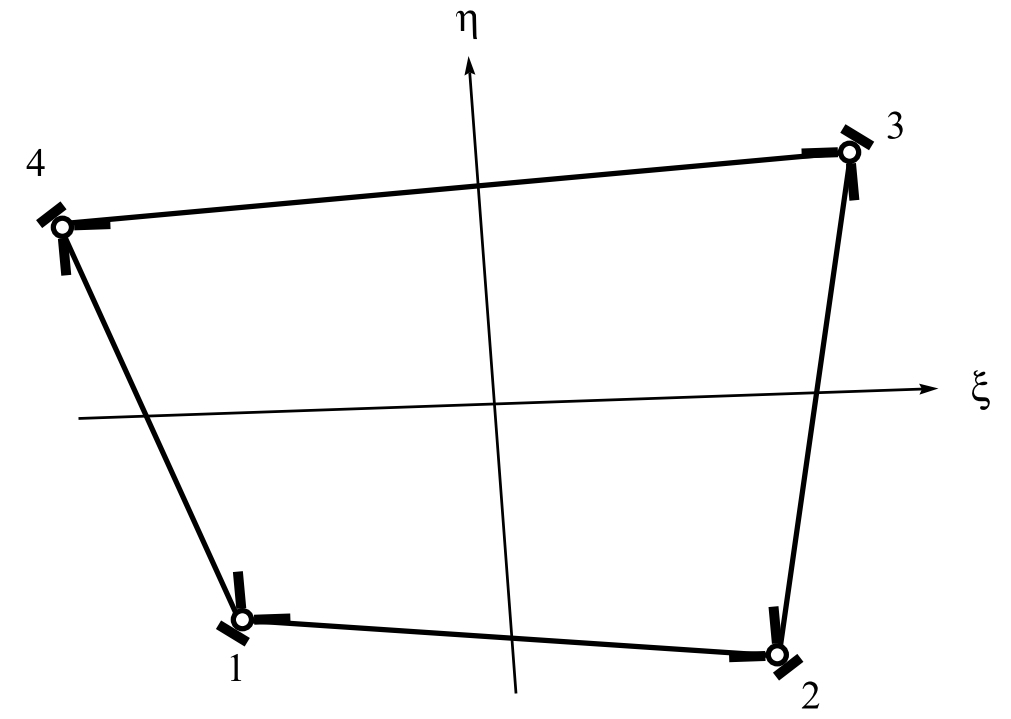
\includegraphics[width=7.3cm]
		{images/ANDES_strain_gauges.png}
		\captionof{figure}{ANDES membrane nodal strain gauges \cite{Hau94}}
		\label{fig:andes_gauges}
	\end{minipage}%
	\begin{minipage}{.5\textwidth}
		\centering
		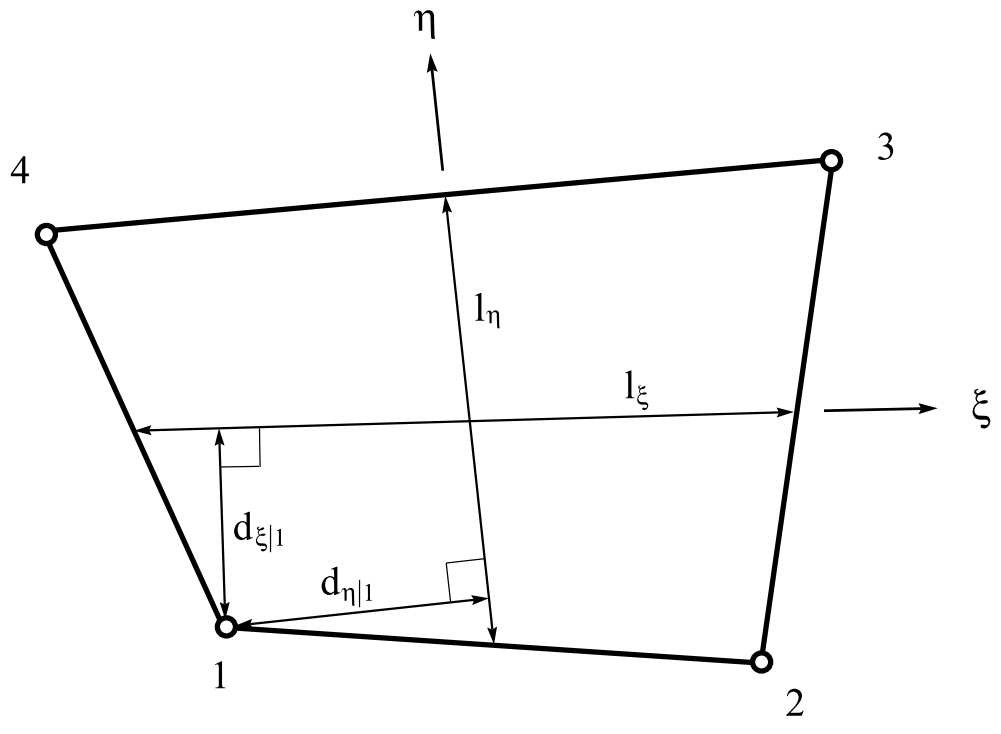
\includegraphics[width=7.3cm]
		{images/andes_geometric_quantities.png}
		\captionof{figure}{Geometric dimensions of the quadrilateral element \cite{Hau94}}
		\label{fig:andes_dims}
	\end{minipage}
\end{figure}

The strain gauges are placed as per figure \ref{fig:andes_gauges} and read strains along the $\xi$ and $\eta$ axes as well as the element diagonals. At each strain gauge, the readings are thus:

\begin{equation} 
\boldsymbol{\epsilon}_{1} = \boldsymbol{\epsilon}_{3} =
\begin{pmatrix}
\epsilon_\xi \\
\epsilon_\eta \\
\epsilon_{24}
\end{pmatrix}
\ ,
\hspace{10mm}
\boldsymbol{\epsilon}_{2} = \boldsymbol{\epsilon}_{4} =
\begin{pmatrix}
\epsilon_\xi \\
\epsilon_\eta \\
\epsilon_{13}
\end{pmatrix}
\label{eqnAndesStrainGauges}
\end{equation}

The strain readings are related to the higher order degrees of freedom via the nodal strain templates $\mathbf{Q}_i$.
\begin{equation} 
\boldsymbol{\epsilon}_{i} = \mathbf{Q}_i \widetilde{\mathbf{v}}
\label{eqnAndesHigherOrderStrains}
\end{equation}

\textit{Higher order bending field}

As per Haugen's PhD thesis, the primary strain mode the field is trying to match is pure bending of an element in an arbitrary direction. The bending strain field is associated with the higher order DOFs of $\theta_i^{'}, \widetilde{v}_{\xi}$ and $\widetilde{v}_{\eta}$, and is intuited to be proportional to the distance from the neutral axis of the direction considered. For instance, bending in the $\xi$ direction is assumed proportional to the distance $d_{\xi}$ (refer figure \ref{fig:andes_dims}) and the curvature of the element $\frac{\Delta \theta}{l_{\xi}}$. Thus the general form of the $\xi$ strains are $\frac{d_{\xi | i}}{l_\xi}$, with the $\eta$ strains derived in a similar manner. The bending strains at each node are:

\begin{equation} 
\chi_{\xi | i} = \frac{d_{\xi | i}}{l_\xi},
\hspace{10mm}
\chi_{\eta | i} = \frac{d_{\eta | i}}{l_\eta},
\label{equation12}
\end{equation}
where the quantities in figure \ref{fig:andes_dims} are calculated as follows:
\begin{align*} 
	d_{\xi | i} = \sqrt{(\mathbf{r}_i \times \mathbf{s_\xi}) \cdot (\mathbf{r}_i \times \mathbf{s_\xi})}\ ,
	\hspace{10mm}
	l_\xi = \sqrt{\mathbf{r_\xi} \cdot \mathbf{r_\xi}}\ ,
	\hspace{10mm} 
	\mathbf{r_\xi} = \frac{1}{2} ( \mathbf{r}_2 + \mathbf{r}_3 - \mathbf{r}_1 - \mathbf{r}_4 )\ , \\
	d_{\eta | i} = \sqrt{(\mathbf{r}_i \times \mathbf{s_\eta}) \cdot (\mathbf{r}_i \times \mathbf{s_\eta})}\ ,
	\hspace{10mm}
	l_\xi = \sqrt{\mathbf{r_\eta} \cdot \mathbf{r_\eta}}\ ,
	\hspace{10mm}
	\mathbf{r_\eta} = \frac{1}{2} ( \mathbf{r}_2 + \mathbf{r}_3 - \mathbf{r}_1 - \mathbf{r}_4 )\ ,
\end{align*}

$\mathbf{s}_\xi$ and $\mathbf{s}_\eta$ are the normalized parametric base vectors in cartesian coordinates, while $\mathbf{r}_i$ are the nodal position vectors in cartesian coordinates.

The diagonal strain components of the higher order bending field are also assumed as to be proportional to the distance and curvature along the diagonal, thus yielding:  

\begin{equation} 
\chi_{24} = \frac{d_{24}}{2 l_{24}},
\hspace{10mm}
\chi_{13} = \frac{d_{13}}{2 l_{13}},
\label{equation12chi24}
\end{equation}
where
\begin{align*} 
\begin{split}
	d_{24} = d_{13} = & \sqrt{(\mathbf{r}_{31} \times \mathbf{e}_{24}) \cdot (\mathbf{r}_{31} \times \mathbf{e}_{24})} \hspace{10mm}
	l_{24} = \sqrt{\mathbf{r}_{24} \cdot \mathbf{r}_{24}}\ ,
	\hspace{10mm}
	\mathbf{r}_{24} = \mathbf{r}_2 - \mathbf{r}_4 \\
	& l_{13} = \sqrt{\mathbf{r}_{13} \cdot \mathbf{r}_{13}}\ ,
	\hspace{10mm}
	\mathbf{r}_{13} = \mathbf{r}_1 - \mathbf{r}_3
	\hspace{10mm}
	\mathbf{e}_{24} = \frac{\mathbf{r}_{24}}{l_{24}}
	\end{split}
\end{align*}

\textit{Higher order torsional field}

The higher order torsional field is associated with the $\bar{\theta}$ higher order DOF. Figure \ref{fig:AndesTorsional} illustrates the general torsional displacement mode shape, indicating that no shear strains are produced in this mode.

\begin{figure}[H]
	\centering
	\def\svgwidth{\columnwidth}
	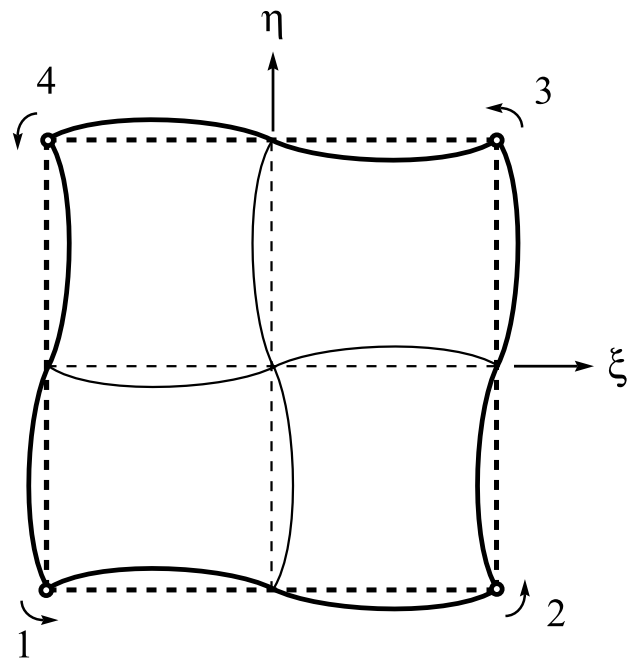
\includegraphics[width=7.3cm]{images/ANDES_torsional_mode.png}
	\caption{Higher order torsional mode of ANDES membrane formulation \cite{Hau94}}
	\label{fig:AndesTorsional}
\end{figure}

Under this torsional regime, $\epsilon_\xi$ is positive in the 1st and 3rd quadrants and negative in the 2nd and 4th quadrants, while $\epsilon_\eta$ has the opposite signs. Furthermore, with a unit rotation at each node the maximum displacement $v_\xi$ will be proportional to $l_\eta$. Recalling that $\epsilon_{\xi}$ is the gradient of $v_\xi$ in the $\xi$ direction, one can suppose that $\epsilon_{\xi}$ is proportional to $\frac{1}{l_\xi}$. Considering this approach for $\epsilon_{\xi}$ and $\epsilon_{\eta}$, the following torsional strain field terms are determined:

\begin{equation} 
\chi_{\xi t} = \frac{l_\eta}{l_\xi}\ ,
\hspace{10mm}
\chi_{\eta t} = \frac{l_\xi}{l_\eta}\ ,
\label{equation13}
\end{equation}

\textit{Higher order nodal strain templates}

Considering the higher order bending and torsional components just outlined, the nodal strain gauge readings can be described as follows:
\begin{equation} 
\mathbf{Q}_1 =
\begin{pmatrix}
\rho_1 \chi_{\xi | 1} & \rho_2 \chi_{\xi | 1} & \rho_3 \chi_{\xi | 1} & \rho_4 \chi_{\xi | 1} & \alpha \chi_{\xi t} & -\beta_1 \frac{\chi_{\xi | 1}}{\bar{\chi_\xi} l_\xi} & 0  \\	
-\rho_1 \chi_{\eta | 1} & -\rho_4 \chi_{\eta | 1} & -\rho_3 \chi_{\eta | 1} & -\rho_2 \chi_{\eta | 1} & -\alpha \chi_{\eta t} & 0 & -\beta_1 \frac{\chi_{\eta | 1}}{\bar{\chi_\eta} l_\eta} \\
\rho_5 \chi_{24} & \rho_6 \chi_{24} & \rho_7 \chi_{24} & \rho_8 \chi_{24} & 0 & \beta_2 \frac{c_{24 \xi}}{l_{24}} & -\beta_2 \frac{c_{24 \eta}}{l_{24}}
\end{pmatrix}		
\label{equation14}
\end{equation}

\begin{equation} 
\mathbf{Q}_2 =
\begin{pmatrix}
-\rho_2 \chi_{\xi | 2} & -\rho_1 \chi_{\xi | 2} & -\rho_4 \chi_{\xi | 2} & -\rho_3 \chi_{\xi | 2} & -\alpha \chi_{\xi t} & -\beta_1 \frac{\chi_{\xi | 2}}{\bar{\chi_\xi} l_\xi} & 0  \\	
\rho_4 \chi_{\eta | 2} & \rho_1 \chi_{\eta | 2} & \rho_2 \chi_{\eta | 2} & \rho_3 \chi_{\eta | 2} & \alpha \chi_{\eta t} & 0 & \beta_1 \frac{\chi_{\eta | 2}}{\bar{\chi_\eta} l_\eta} \\
\rho_8 \chi_{13} & \rho_5 \chi_{13} & \rho_6 \chi_{13} & \rho_7 \chi_{13} & 0 & -\beta_2 \frac{c_{13 \xi}}{l_{13}} & \beta_2 \frac{c_{13 \eta}}{l_{13}}
\end{pmatrix}		
\label{equation14_2}
\end{equation}

\begin{equation} 
\mathbf{Q}_3 =
\begin{pmatrix}
\rho_3 \chi_{\xi | 3} & \rho_4 \chi_{\xi | 3} & \rho_1 \chi_{\xi | 3} & \rho_2 \chi_{\xi | 3} & \alpha \chi_{\xi t} & \beta_1 \frac{\chi_{\xi | 3}}{\bar{\chi_\xi} l_\xi} & 0  \\	
-\rho_3 \chi_{\eta | 3} & -\rho_2 \chi_{\eta | 3} & -\rho_1 \chi_{\eta | 3} & -\rho_4 \chi_{\eta | 3} & -\alpha \chi_{\eta t} & 0 & \beta_1 \frac{\chi_{\eta | 3}}{\bar{\chi_\eta} l_\eta} \\
\rho_7 \chi_{13} & \rho_8 \chi_{13} & \rho_5 \chi_{13} & \rho_6 \chi_{213} & 0 & -\beta_2 \frac{c_{13 \xi}}{l_{13}} & \beta_2 \frac{c_{13 \eta}}{l_{13}}
\end{pmatrix}		
\label{equation14_3}
\end{equation}

\begin{equation} 
\mathbf{Q}_4 =
\begin{pmatrix}
-\rho_4 \chi_{\xi | 4} & -\rho_3 \chi_{\xi | 4} & -\rho_2 \chi_{\xi | 4} & -\rho_1 \chi_{\xi | 4} & -\alpha \chi_{\xi t} & \beta_1 \frac{\chi_{\xi | 4}}{\bar{\chi_\xi} l_\xi} & 0  \\	
\rho_2 \chi_{\eta | 4} & \rho_3 \chi_{\eta | 4} & \rho_4 \chi_{\eta | 4} & \rho_1 \chi_{\eta | 4} & \alpha \chi_{\eta t} & 0 & -\beta_1 \frac{\chi_{\eta | 4}}{\bar{\chi_\eta} l_\eta} \\
\rho_6 \chi_{13} & \rho_7 \chi_{13} & \rho_8 \chi_{13} & \rho_5 \chi_{13} & 0 & \beta_2 \frac{c_{13 \xi}}{l_{13}} & -\beta_2 \frac{c_{13 \eta}}{l_{13}}
\end{pmatrix}		
\label{equation15}
\end{equation}
where
\begin{align*} 
	c_{13 \xi} = \mathbf{s}_{13}^T \mathbf{s_\xi}\ ,
	\hspace{10mm}
	c_{13 \eta} = \mathbf{s}_{13}^T \mathbf{s_\eta}\ ,
	\hspace{10mm}
	c_{24 \xi} = \mathbf{s}_{24}^T \mathbf{s_\xi}\ ,
	\hspace{10mm}
	c_{24 \eta} = \mathbf{s}_{24}^T \mathbf{s_\eta}
	\hspace{10mm}
\end{align*}

An optimisation of element performance has suggested the following coefficients to be used in the nodal strain gauge templates \cite{Hau94}. 
\begin{gather} 
	\begin{aligned}
		&\rho_1 = 0.1\ ,
		\hspace{10mm}
		\rho_2 = -0.1\ ,
		\hspace{10mm}
		\rho_3 = -0.1\ ,
		\hspace{10mm}
		\rho_4 = 0.1\ ,
		\hspace{10mm}
		\rho_5 = 0.0\ , \\
		&\rho_6 = 0.5\ ,
		\hspace{10mm}
		\rho_7 = 0.0\ ,
		\hspace{10mm}
		\rho_8 = -0.5\ ,
		\hspace{10mm}
		\beta_1 = 0.6\ ,
		\hspace{10mm}
		\beta_2 = 0.0
		\label{equation16}
	\end{aligned}
\end{gather}

\textit{Cartesian higher order strain displacement matrix}

The Cartesian strain displacement matrices at the nodes are related to the mapping matrices $\mathbf{Q}_i$ as described below:
\begin{gather} 
	\begin{aligned}
		&\mathbf{B}_{h1} = \mathbf{T}_{13}  \mathbf{Q}_{1}\ ,
		\hspace{10mm}
		\mathbf{B}_{h3} = \mathbf{T}_{13}  \mathbf{Q}_{3}\\
		&where 
		\hspace{10mm} 
		\mathbf{T}_{13}^{-1} =
		\begin{pmatrix}
			s_{\xi x}^2 & s_{\xi y}^2 & s_{\xi x} s_{\xi y} \\
			s_{\eta x}^2 & s_{\eta y}^2 & s_{\eta x} s_{\eta y} \\
			s_{24 x}^2 & s_{24 y}^2 & s_{24 x} s_{24 y}
		\end{pmatrix}
		\label{equation17}
	\end{aligned}
\end{gather}
\begin{gather} 
	\begin{aligned}
		&\mathbf{B}_{h2} = \mathbf{T}_{24}  \mathbf{Q}_{2}\ ,
		\hspace{10mm}
		\mathbf{B}_{h4} = \mathbf{T}_{24}  \mathbf{Q}_{4}\\
		&where 
		\hspace{10mm} 
		\mathbf{T}_{24}^{-1} =
		\begin{pmatrix}
			s_{\xi x}^2 & s_{\xi y}^2 & s_{\xi x} s_{\xi y} \\
			s_{\eta x}^2 & s_{\eta y}^2 & s_{\eta x} s_{\eta y} \\
			s_{13 x}^2 & s_{13 y}^2 & s_{13 x} s_{13 y}
		\end{pmatrix}
		\label{equation18}
	\end{aligned}
\end{gather}

The total higher order membrane B matrix $\mathbf{B}_h$ is constructed from the interpolation of the nodal $\mathbf{B}_{hi}$ matrices with standard bi-linear shape functions.
\begin{equation} 
\mathbf{B}_h(\xi,\eta) = (1-\xi)(1-\eta)\mathbf{B}_{h1} + (1+\xi)(1-\eta)\mathbf{B}_{h2} + (1+\xi)(1+\eta)\mathbf{B}_{h3} +	(1-\xi)(1+\eta)\mathbf{B}_{h4} 
\label{equation19}
\end{equation}

A requirement of the underlying FF is energy orthogonality between the basic and higher order strain fields, which is not yet fulfilled. This orthogonality can be achieved by rendering the higher order field deviatoric, as per the formulation name, which involves subtracting the mean integral:

\begin{equation} 
\mathbf{B}_d(\xi,\eta) = \mathbf{B}_h(\xi,\eta) - \bar{\mathbf{B}}_h
\hspace{10mm}
with
\hspace{10mm}
\bar{\mathbf{B}}_h = \int_A \mathbf{B}_h(\xi,\eta) \ dA
\label{eqnAndesDevB}
\end{equation}

\subsection{DKQ bending formulation}
\label{section:DKQ bending formulation}

The bending formulation is responsible for providing the bending stiffness of the element, with an enhanced formulation selected to pre-empt transverse shear locking. The bending formulation chosen was the Discrete Kirchhoff Quadrilateral (DKQ) formulation  originally presented by Batoz \cite{Bat82}, presented in a most readable fashion in the PhD dissertation of Barrales \cite{Bar12}. A full description and theoretical derivation of the DKQ approach falls outside the scope of this document, refer \cite{Bat82}. As described in section \ref{dkqtheory}, the transverse shear strain energy is neglected which prohibits element performance deterioration as the ratio $\frac{l}{t}$ encroaches into thin and very thin plate territories.

Only the bending portion of the total shell element is considered in this section, in which there are three nodal DOFs per node $(w_i$ corresponds to $u_{zi}$ in the figure below).

\begin{figure}[H]
	\centering
	\def\svgwidth{\columnwidth}
	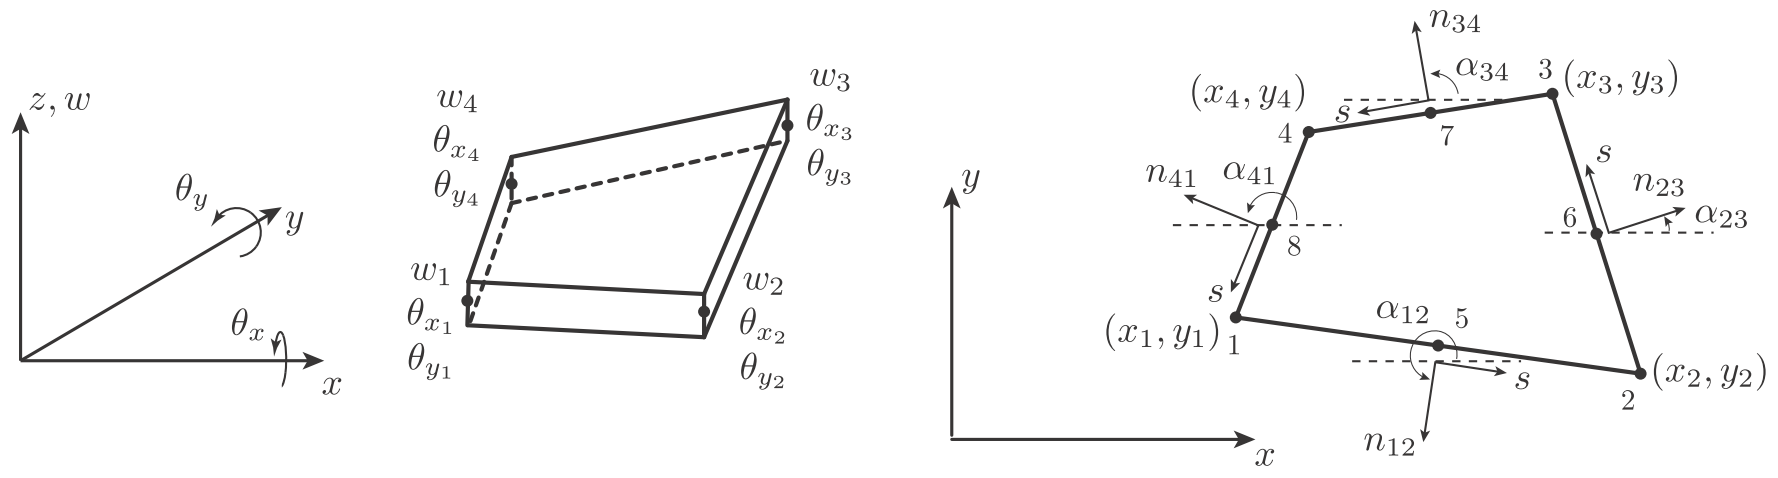
\includegraphics[width=15cm]{images/8nodeseren.png}
	\caption{DKQ DOF arrangement and geometry \cite{Bar12}}
	\label{8nodeseren}
\end{figure}

\begin{equation} 
\mathbf{u}^T = 
\begin{pmatrix}
\mathbf{u}_1 & \mathbf{u}_2 & \mathbf{u}_3 & \mathbf{u}_4
\end{pmatrix} 
\hspace{10mm}
where
\hspace{10mm}
\mathbf{u}{_i}^T = 
\begin{pmatrix}
{u_{zi}} & {\theta_{xi}} & {\theta_{yi}}
\end{pmatrix}
\label{equationBending}
\end{equation}

The nodal rotational interpolation employed is as per the 8 node serendipity quad element:

\begin{equation} 
\begin{pmatrix}
\beta_x (\xi , \eta) \\
\beta_y (\xi , \eta)
\end{pmatrix}
= \sum_{i=1}^8 \psi_i (\xi , \eta) 
\begin{pmatrix}
\beta_{xi} (\xi , \eta) \\
\beta_{yi} (\xi , \eta)
\end{pmatrix}
\label{equation20}
\end{equation}

where $\psi_i$ are the standard 8 node serendipity shape functions described by Zienkiewicz \cite{Zie77}:

\begin{gather} 
	\begin{aligned}
		&\psi_i (\xi , \eta) = \frac{-1}{4} (1 + \xi_i \xi)(1 + \eta_i \eta)(1 - \xi_i \xi - \eta_i \eta)
		\hspace{10mm}
		i = 1, 2, 3, 4 \\
		&\psi_i (\xi , \eta) = \frac{1}{2} (1 - \xi^2)(1 + \eta_i \eta)
		\hspace{10mm}
		i = 5, 7 \\
		&\psi_i (\xi , \eta) = \frac{1}{2} (1 + \xi_i \xi)(1 - \eta^2)
		\hspace{10mm}
		i = 6, 8
		\label{equation21}
	\end{aligned}
\end{gather}

and $\xi_i$ and $\eta_i$ are the natural coordinates of the 8 node serendipity element described in figure \ref{8nodeseren}.

The following derivation from equations \eqref{equation22} to \eqref{equation27} is summarised from that of Barrales \cite{Bar12}. The general idea is the construction of a mapping from the standard 12 DOFs at each node to $\beta_x (\xi,\ \eta)$ and $\beta_y (\xi,\ \eta)$ across the element, the derivatives of which are curvatures as expressed in equation \eqref{equation27}.

The following quantities are required components for the mapping:

\begin{equation} 
L_{ij} = \sqrt{x_{ij}^2 + y_{ij}^2}\ ,
\hspace{10mm}
x_{ij} = x_i - x_j\ ,
\hspace{10mm}
y_{ij} = y_i - y_j
\label{equation22}
\end{equation}
\begin{gather} 
	\begin{aligned}
		&a_k = \frac{-x_{ij}}{L_{ij}^2}\ ,
		\hspace{10mm}
		b_k = \frac{3}{4} \frac{x_{ij} y_{ij}}{L_{ij}^2}\ , \\
		c_k = \frac{\frac{1}{4} x_{ij}^2 - \frac{1}{2} y_{ij}^2}{L_{ij}^2}\
		& ,
		\hspace{10mm}
		d_k = \frac{-y_{ij}}{L_{ij}^2}\ ,
		\hspace{10mm}
		e_k = \frac{\frac{-1}{2} x_{ij}^2 + \frac{1}{4} y_{ij}^2}{L_{ij}^2}
		\label{equation23}
	\end{aligned}
\end{gather}

The elements of the mapping matrix are arranged as such:

\begin{equation} 
\mathbf{\Psi}^x = 
\begin{pmatrix}
\Psi_1^x \\
\vdots \\
\Psi_{12}^x
\end{pmatrix}\ ,
\hspace{10mm}
\mathbf{\Psi}^y = 
\begin{pmatrix}
\Psi_1^y \\
\vdots \\
\Psi_{12}^y
\end{pmatrix}
\label{equation24}
\end{equation}

where the vectors entries are calculated as per the following scheme:
\begin{gather} 
	\begin{aligned}
		&\Psi_{3(i-1)+1}^x (\xi , \eta) = \frac{3}{2} (a_r \psi_r (\xi , \eta) - a_s \psi_s (\xi , \eta) ) \\
		&\Psi_{3(i-1)+2}^x (\xi , \eta) = b_r \psi_r (\xi , \eta) + b_s \psi_s (\xi , \eta) \\
		&\Psi_{3(i-1)+3}^x (\xi , \eta) = \psi_i (\xi , \eta) - c_r \psi_r (\xi , \eta) - c_s \psi_s (\xi , \eta)
		\label{equation25}
	\end{aligned}
\end{gather}
\begin{gather} 
	\begin{aligned}
		&\Psi_{3(i-1)+1}^y (\xi , \eta) = \frac{3}{2} (d_r \psi_r (\xi , \eta) - d_s \psi_s (\xi , \eta) ) \\
		&\Psi_{3(i-1)+2}^y (\xi , \eta) = -\psi_i (\xi , \eta) + e_r \psi_r (\xi , \eta) + c_s \psi_s (\xi , \eta) \\
		&\Psi_{3(i-1)+3}^y (\xi , \eta) = -b_r \psi_r (\xi , \eta) - b_s \psi_s (\xi , \eta)
		\label{equation26}
	\end{aligned}
\end{gather}

with $i$ = 1, 2, 3, 4 and the relationship $(i,\ r,\ s)$ as (1, 5, 8), (2, 6, 5), (3, 7, 6) and (4, 8, 7).

Relating curvatures to displacements yield:

\begin{equation} 
\boldsymbol{\chi} = \mathbf{B}_{bend} \mathbf{U}
\label{equation27}
\end{equation}

with $\mathbf{B}_{bend}$ constructed as follows:

\begin{equation} 
\mathbf{B}_{bend} =
\begin{pmatrix}
\frac{\partial \mathbf{\Psi}^{x^T}}{\partial x} \\
\frac{\partial \mathbf{\Psi}^{y^T}}{\partial y} \\
\frac{\partial \mathbf{\Psi}^{x^T}}{\partial y} + \frac{\partial \mathbf{\Psi}^{y^T}}{\partial x}
\end{pmatrix}
\ =\ 
\begin{pmatrix}
j_{11} \frac{\partial \mathbf{\Psi}^{x^T}}{\partial \xi}  + j_{12} \frac{\partial \mathbf{\Psi}^{x^T}}{\partial \eta}  \\
j_{21} \frac{\partial \mathbf{\Psi}^{y^T}}{\partial \xi} + j_{22} \frac{\partial \mathbf{\Psi}^{y^T}}{\partial \eta} \\
j_{11} \frac{\partial \mathbf{\Psi}^{y^T}}{\partial \xi}  + j_{12} \frac{\partial \mathbf{\Psi}^{y^T}}{\partial \eta} + j_{21} \frac{\partial \mathbf{\Psi}^{x^T}}{\partial \xi} + j_{22} \frac{\partial \mathbf{\Psi}^{x^T}}{\partial \eta}
\end{pmatrix}
\label{equation28}
\end{equation}

and the inverse Jacobian entries $j_{\alpha \beta}$:
\begin{gather} 
	\begin{aligned}
		&\mathbf{J} = \frac{1}{4}
		\begin{pmatrix}
			x_{21} + x_{34} + \eta (x_{12} + x_{34}) & y_{21} + y_{34} + \eta (y_{12} + y_{34}) \\
			x_{32} + x_{41} + \xi (x_{12} + x_{34}) & y_{32} + y_{41} + \xi (y_{12} + y_{34})
		\end{pmatrix}
		\ = \ 
		\begin{pmatrix}
			J_{11} & J_{12} \\
			J_{21} & J_{22}
		\end{pmatrix} \\
		&j_{11} = \frac{J_{22}}{det[J]}\ ,
		\hspace{10mm}
		j_{12} = \frac{-J_{12}}{det[J]}\ ,
		\hspace{10mm}
		j_{21} = \frac{-J_{21}}{det[J]}\ ,
		\hspace{10mm}
		j_{22} = \frac{J_{11}}{det[J]}
		\label{equation29}
	\end{aligned}
\end{gather}

\subsection{Combined formulation}

With the separate membrane and bending B matrices developed, the combined shell B matrix $\mathbf{B}_{comb.}$ can be constructed to form the element stiffness matrix.

\begin{equation} 
\mathbf{K}_{el} = \mathbf{B}_{comb}^T \mathbf{C} \mathbf{B}_{comb} 
\label{equation30}
\end{equation}

\begin{equation} 
\mathbf{B}_{comb} = (\mathbf{L} + \mathbf{B}_h) + \mathbf{B}_{bend} = \mathbf{B}_{mem} + \mathbf{B}_{bend} = 
\begin{pmatrix}
\mathbf{B}_{comb1} & \mathbf{B}_{comb2} & \mathbf{B}_{comb3} & \mathbf{B}_{comb4}
\end{pmatrix}
\label{equation31}
\end{equation}

The combination of $\textcolor{blue}{membrane}$ and $\textcolor{red}{bending}$ matrices must consider the DOF ordering of each component and the relation to the total shell DOF ordering, as shown below:

\begin{equation} 
\mathbf{u}_i = 
\begin{pmatrix}
\textcolor{blue}{u_{xi}} \\ 
\textcolor{blue}{u_{yi}} \\ 
\textcolor{red}{u_{zi}} \\ 
\textcolor{red}{\beta_{xi}} \\ 
\textcolor{red}{\beta_{yi}} \\ 
\textcolor{blue}{\beta_{zi}} \\ 
\end{pmatrix}
\label{equation32}
\end{equation}

Considering this, the addition of the membrane (basic and higher order) B matrices and the bending B matrix is conducted for each node \textit{i} as follows:

\begin{multline}
	\mathbf{B}_{comb\ i} = \left(
	\begin{matrix}
		\textcolor{blue}{\mathbf{B}_{mem}[1,3(i-1) + 1]} & \textcolor{blue}{\mathbf{B}_{mem}[1,3(i-1) + 2]} & 0 \\ 
		\textcolor{blue}{\mathbf{B}_{mem}[2,3(i-1) + 1]} & \textcolor{blue}{\mathbf{B}_{mem}[2,3(i-1) + 2]} & 0 \\ 
		0 & 0 & \textcolor{red}{\mathbf{B}_{bend}[1,3(i-1) + 1]} \\ 
		0 & 0 & \textcolor{red}{\mathbf{B}_{bend}[2,3(i-1) + 1]} \\
		0 & 0 & \textcolor{red}{\mathbf{B}_{bend}[3,3(i-1) + 1]} \\
		\textcolor{blue}{\mathbf{B}_{mem}[3,3(i-1) + 1]} & \textcolor{blue}{\mathbf{B}_{mem}[3,3(i-1) + 2]} & 0 \\
	\end{matrix}\right.                
	\\
	\left.
	\begin{matrix}
		0 & 0 & \textcolor{blue}{\mathbf{B}_{mem}[1,3(i-1) + 3]} \\ 
		0 & 0 & \textcolor{blue}{\mathbf{B}_{mem}[2,3(i-1) + 3]} \\ 
		\textcolor{red}{\mathbf{B}_{bend}[1,3(i-1) + 2]} & \textcolor{red}{\mathbf{B}_{bend}[1,3(i-1) + 3]} & 0 \\ 
		\textcolor{red}{\mathbf{B}_{bend}[2,3(i-1) + 2]} & \textcolor{red}{\mathbf{B}_{bend}[2,3(i-1) + 3]} & 0 \\
		\textcolor{red}{\mathbf{B}_{bend}[3,3(i-1) + 2]} & \textcolor{red}{\mathbf{B}_{bend}[3,3(i-1) + 3]} & 0 \\
		0 & 0 & \textcolor{blue}{\mathbf{B}_{mem}[3,3(i-1) + 3]} \\
	\end{matrix}\right)
	\label{equation33}
\end{multline}

\section{Stiffness matrix implementation}

With the formulation of the ANDES-DKQ shell element established, a high level overview of it's implementation in KRATOS is discussed in this section.

The new quad element is implemented in the files $\texttt{shell\_thin\_element\_3D4N.hpp}$ and\break$\texttt{shell\_thin\_element\_3D4N.cpp}$, which are compiled into the 'StructuralMechanicsApplication' module of Kratos. Similar to the DSG triangle element, the new ANDES-DKQ element class $\texttt{ShellThinElement3D4N}$ is inherited from the Kratos base class $\texttt{Element}$ and also leverages the existing capabilities other Kratos classes offer. The general workflow of calculating the ANDES-DKQ stiffness matrix is as follows:

\begin{figure}[H]
	% Define block styles
	\tikzstyle{virtual} = [rectangle, minimum width=3cm, minimum height=1cm, text centered, draw=black, fill=orange!30]
	\tikzstyle{process} = [rectangle, minimum width=3cm, minimum height=1cm, text centered, draw=black, fill=white!30]
	\tikzstyle{arrow} = [thick,->,>=stealth]
	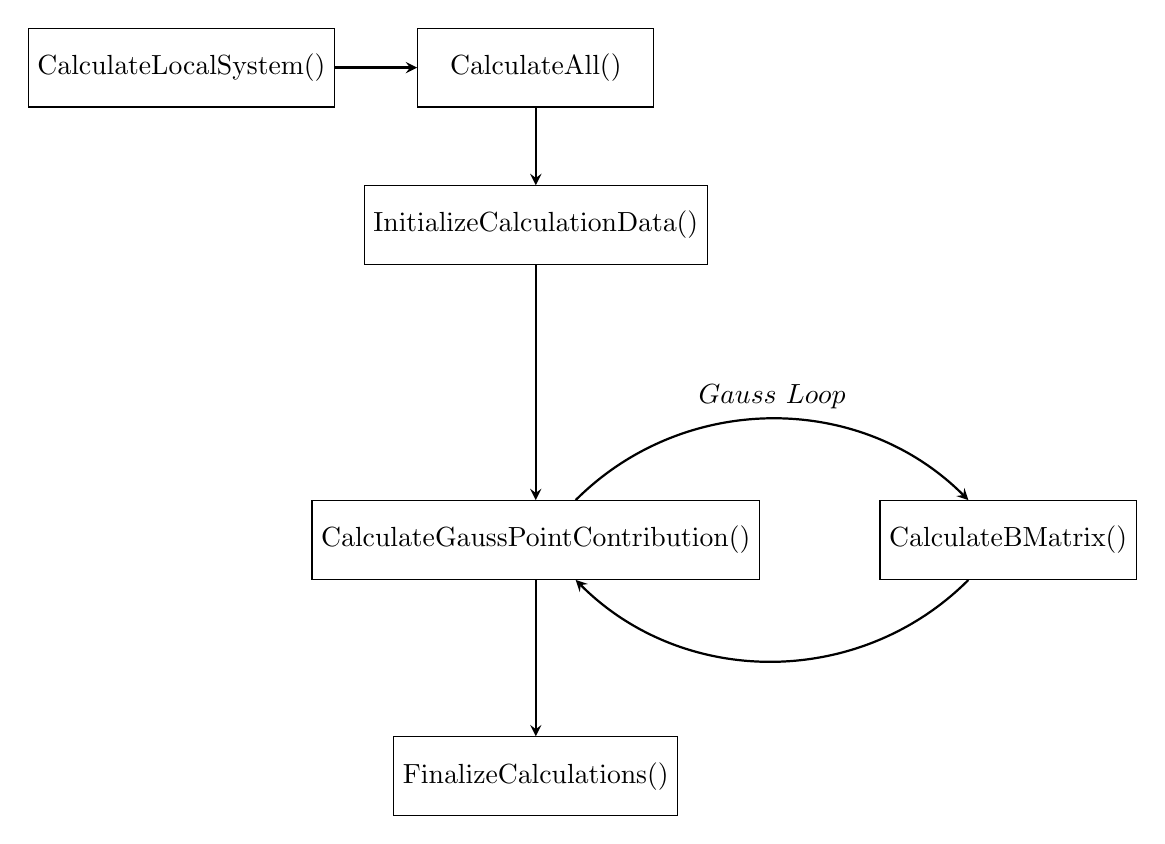
\begin{tikzpicture}[node distance = 2cm, auto]
	% Place nodes
	\node [process] (CalculateLocalSystem) {CalculateLocalSystem()};
	\node [process, right of=CalculateLocalSystem, xshift = 2.5cm] (CalculateAll) {CalculateAll()};
	\node [process, below of=CalculateAll, xshift = -0cm] (InitializeCalculationData) {InitializeCalculationData()};
	\node [process, below of=InitializeCalculationData, yshift = -2cm] (CalculateGaussPointContribution) {CalculateGaussPointContribution()};
	\node [process, right of=CalculateGaussPointContribution, xshift = 4cm] (CalculateBMatrix) {CalculateBMatrix()};
	\node [process, below of=CalculateGaussPointContribution, yshift = -1cm] (FinalizeCalculations) {FinalizeCalculations()};
	% Draw edges
	\draw [arrow] (CalculateLocalSystem) -- (CalculateAll);
	\draw [arrow] (CalculateAll) -- (InitializeCalculationData);
	\draw [arrow] (InitializeCalculationData) -- (CalculateGaussPointContribution);
	\draw [arrow] (CalculateGaussPointContribution) -- (FinalizeCalculations);
	\draw [arrow] (CalculateGaussPointContribution) edge[bend left=45] node [above] {$Gauss\ Loop$} (CalculateBMatrix);
	\draw [arrow] (CalculateBMatrix) edge[bend left=45] node [below] {} (CalculateGaussPointContribution);
	\end{tikzpicture}
	\caption{High level overview of ANDES-DKQ element workflow}
	\label{andesworkflow}
\end{figure}

As per the DSG triangle element, the re-implemented virtual method $\texttt{CalculateLocalSystem()}$ is called by the KRATOS framework automatically for every $\texttt{ShellThinElement3D4N}$ in the job definition. This method simply calls $\texttt{CalculateAll()}$, which initializes calculating the stiffness matrix by calling $\texttt{InitializeCalculationData(),\ CalculateGaussPointContribution()}$ and $\texttt{FinalizeCalculations()}$.

$\texttt{InitializeCalculationData()}$ is called first, and pre-calculates quantities so they can be removed from the Gauss loop. These quantities include the ANDES basic lumping matrix $\textbf{L}$, the ANDES higher order strain-displacement matrices $\textbf{B}_{hi}$ and all DKQ coefficients in equation  \eqref{equation23}.

$\texttt{CalculateAll()}$ then calls $\texttt{CalculateGaussPointContribution()}$ which starts the Gauss integration loop. At each Gauss point $\texttt{CalculateGaussPointContribution()}$ performs Gauss integration of the expression $\textbf{K}_{contribution}$ = $\textbf{B}_{comb}^T \textbf{C} \textbf{B}_{comb}\  dA$, with the current $\textbf{B}_{comb}$ determined by calling $\texttt{CalculateBMatrix()}$.

With the Gauss integration complete, $\texttt{CalculateAll()}$ lastly calls $\texttt{FinalizeCalculations()}$ which transforms the calculated element stiffness from local to global coordinates.

The following pseudocode summarises the key calls and operations involved in calculating the ANDES-DKQ element stiffness matrix.

\begin{algorithm}
	\onehalfspacing
	\caption{ANDES-DKQ element stiffness matrix pseudocode}\label{ANDES-DKQ element stiffness matrix}
	\begin{algorithmic}[1]
		\Require Coordinate transformation instance
		\State \textbf{call} $\texttt{CalculateAll()}$
		\State Resize $LHS$ and $RHS$
		\State \textbf{call} $\texttt{InitializeCalculationData}(data)$
		\State \hspace{\algorithmicindent}Calculate integration areas $dA = w_i \cdot detJ(xi,\ eta)$
		\State \hspace{\algorithmicindent}Determine basic membrane strain displacement $L$
		\State \hspace{\algorithmicindent}Construct membrane higher order filter matrix $H$
		\State \hspace{\algorithmicindent}Arrange higher order natural strain matrices $Q_i$
		\State \hspace{\algorithmicindent}Transform $Q_i$ into $B_{hi}$
		\State \hspace{\algorithmicindent}Determine $\bar{B_h}$
		\State \hspace{\algorithmicindent}Pre-calculate all DKQ coefficients
		\While{$gaussPoint$ < 4}
		\State \textbf{call} $\texttt{CalculateGaussPointContribution}(data)$
		\State \hspace{\algorithmicindent}\textbf{call} $\texttt{CalculateBMatrix}(data)$
		\State \hspace{\algorithmicindent}\hspace{\algorithmicindent} Calculate and combine $B_{mem}$ and $B_{bend}$ into $B$
		\State \hspace{\algorithmicindent}\textbf{call} $\texttt{CalculateSectionResponse}(data)$
		\State \hspace{\algorithmicindent}\hspace{\algorithmicindent} Calculate material properties $C$
		\State \hspace{\algorithmicindent}Add stiffness matrix Gauss point contribution to $LHS$
		\EndWhile
		\State Modify $RHS$ residual vector
		\State \textbf{call} $\texttt{FinalizeCalculations}(data,\ displacements,\ LHS,\ RHS)$
		\State \textbf{call} $\texttt{AddBodyForces}(data,\ RHS)$
	\end{algorithmic}
\end{algorithm}

\section{Mass matrix formulation}

The mass matrix is necessary to facilitate dynamic analysis with the thin quadrilateral shell element. Both lumped and consistent options have been implemented.

\subsection{Lumped mass matrix}
The lumped mass matrix is the default option used due to it's speed of construction without significant loss of accuracy. The general form of the ANDES-DKQ lumped matrix is similar to the DSG lumped matrix.
\begin{equation} 
\mathbf{M} =  
\begin{pmatrix}
\mathbf{M}_1 & \mathbf{0} & \mathbf{0} & \mathbf{0}\\
\mathbf{0} & \mathbf{M}_2 & \mathbf{0} & \mathbf{0}\\
\mathbf{0} & \mathbf{0} & \mathbf{M}_3 & \mathbf{0}\\
\mathbf{0} &\mathbf{0} & \mathbf{0} & \mathbf{M}_4
\end{pmatrix}
\hspace{10mm}
where
\hspace{10mm}
\mathbf{M}_i =  
\begin{pmatrix}
\bar{m} & 0 & 0 & 0 & 0 & 0\\
0 & \bar{m} & 0 & 0 & 0 & 0\\
0 & 0 & \bar{m} &0 & 0 & 0\\
0 & 0 & 0 & 0 & 0 & 0\\
0 & 0 & 0 & 0 & 0 & 0\\
0 & 0 & 0 & 0 & 0 & 0
\end{pmatrix}
\label{eqqmass1}
\end{equation}

The general lumped mass is determined for a multi-ply material with $n$ plies each of $t_i$ thickness and $\rho_i$ density as follows:

\begin{equation} 
\bar{m} = \frac{A}{4} \sum_{i=1}^n \rho_i h_i
\label{eqqmass2}
\end{equation}

For a single layer material of area $A$ this reduces to:

\begin{equation} 
\bar{m} = \frac{A}{4} \rho h
\label{eqqmass3}
\end{equation}

\subsection{Consistent mass matrix}
A consistent mass matrix is also provided, and once again has a similar form to the DSG consistent mass matrix. The continuous form for a shell with constant thickness is re-written below for clarity:

\begin{equation} 
\mathbf{M}_C
=
h
\int_{\Omega} 
\rho 
\Big[
\mathbf{N}_T^T
\mathbf{N}_T
+
\frac{h^2}{12}
\mathbf{N}_R^T
\mathbf{N}_R
\Big]
\ d\Omega
\label{eqqmass4}
\end{equation}

For the quadrilateral element, the nodal shape function matrices are expanded from 3 nodes to 4 nodes:

\begin{equation} 
\mathbf{N}_T = 
\begin{pmatrix}
\mathbf{N}_{T_1} & \mathbf{N}_{T_2} & \mathbf{N}_{T_3} & \mathbf{N}_{T_4}
\end{pmatrix}\ ,
\hspace{10mm}
\mathbf{N}_R = 
\begin{pmatrix}
\mathbf{N}_{R_1} & \mathbf{N}_{R_2} & \mathbf{N}_{R_3} & \mathbf{N}_{R_4}
\end{pmatrix}
\label{eqqmass5}
\end{equation}
\begin{equation} 
\mathbf{N}_{T_i} = 
\begin{pmatrix}
N_i & 0 & 0 & 0 & 0 & 0 & 0 & 0\\
0 & N_i & 0 & 0 & 0 & 0 & 0 & 0\\
0 & 0 & N_i & 0 & 0 & 0 & 0 & 0\\
0 & 0 & 0 & N_i & 0 & 0 & 0 & 0\\
0 & 0 & 0 & 0 & 0 & 0 & 0 & 0\\
0 & 0 & 0 & 0 & 0 & 0 & 0 & 0\\
0 & 0 & 0 & 0 & 0 & 0 & 0 & 0\\
0 & 0 & 0 & 0 & 0 & 0 & 0 & 0
\end{pmatrix}
\hspace{10mm}
\mathbf{N}_{R_i} = 
\begin{pmatrix}
0 & 0 & 0 & 0 & 0 & 0 & 0 & 0\\
0 & 0 & 0 & 0 & 0 & 0& 0 & 0\\
0 & 0 & 0 & 0 & 0 & 0 & 0 & 0\\
0 & 0 & 0 & 0 & 0 & 0 & 0 & 0\\
0 &0 & 0 & 0 & N_i & 0 & 0  & 0\\
0 &0 & 0 & 0 & 0 & N_i & 0  & 0\\
0 &0 & 0 & 0 & 0 & 0 & N_i  & 0\\
0 &0 & 0 & 0 & 0 & 0 & 0 & \alpha N_i
\end{pmatrix}
\label{eqqmass5_1}
\end{equation}

Unlike the DSG element which could be evaluated directly, the consistent mass matrix of the ANDES-DKQ is evaluated with numerical 2x2 Gauss integration. Thus, equation \ref{eqqmass4} can be equivalently written in parametric space:

\begin{equation} 
\mathbf{M}_C
=
h
\int_{-1}^{1} 
\int_{-1}^{1} 
\rho 
\Big[
\mathbf{N}_T^T
\mathbf{N}_T
+
\frac{h^2}{12}
\mathbf{N}_R^T
\mathbf{N}_R
\Big]
\ d\eta
\ d\xi
\ det (\mathbf{J})
\label{eqqmass6}
\end{equation}

Shifting over to Gauss integration, the consistent mass matrix is determined numerically from:
\begin{equation} 
\mathbf{M}_C
=
h
\sum_{i=1}^{4 GP}
\rho(\xi_{i},\eta_{i})
\Big[
\mathbf{N}_T^T(\xi_{i},\eta_{i})
\mathbf{N}_T(\xi_{i},\eta_{i})
+
\frac{h^2}{12}
\mathbf{N}_R^T(\xi_{i},\eta_{i})
\mathbf{N}_R(\xi_{i},\eta_{i})
\Big]
w_i
\ det (\mathbf{J}(\xi_{i},\eta_{i}))
\label{eqqmass7}
\end{equation}

\section{Stress and strain recovery}

The stresses and strains of the ANDES-DKT quadrilateral element are recovered in a similar way to the DSG triangle, with the added complication of the multiple Gauss points.

The non-zero local strains ($\epsilon_{zz},\ \epsilon_{xz},\ \epsilon_{yz} = 0$) of the 4 noded 3 parameter element can be arranged in a vector form:
\begin{equation} 
\boldsymbol{\epsilon}^T = \begin{pmatrix}
\boldsymbol{\epsilon}_1 & \boldsymbol{\epsilon}_2 & \boldsymbol{\epsilon}_3 & \boldsymbol{\epsilon}_4
\end{pmatrix}
\hspace{5mm}
with
\hspace{5mm}
\boldsymbol{\epsilon}^T_i = \begin{pmatrix}
\epsilon_{xx} & \epsilon_{xx} & 2\epsilon_{xy} & \epsilon_{xx} & \kappa_{xx} & \kappa_{yy} & 2\kappa_{xy} 
\end{pmatrix}
\label{eqqrec1}
\end{equation}

The nodal strain vector is recovered from the displacement field by applying the strain displacement matrix, which varies over the element.

\begin{equation} 
\boldsymbol{\epsilon}(\xi,\ \eta) = \mathbf{B}(\xi,\ \eta) \mathbf{u}(\xi,\ \eta)
\label{eqqrec2}
\end{equation}

As per the DSG triangle, the strains and stresses are calculated at the Gauss points of the element, with the ANDES-DKT element having four Gauss points ($j = 1,\ 2,\ 3,\ 4$). Thus, the strain vector at each Gauss point $j$ is recovered from the discrete nodal displacements $\hat{\mathbf{u}}_i$ as follows:

\begin{equation} 
\boldsymbol{\epsilon}_{GP_j} = \mathbf{B}(\xi_j,\ \eta_j) \sum_{i=1}^{4\ nodes} N_i(\xi_j,\ \eta_j) \hat{\mathbf{u}}_i
\label{eqqrec3}
\end{equation}

With the strains determined, the stresses at each Gauss point are recovered with the material matrix (which in the general case may vary over the element).

\begin{equation} 
\boldsymbol{\sigma}_{GP_j} = \mathbf{C}_{GP_j}\ \boldsymbol{\epsilon}_{GP_j}
\label{eqqrec4}
\end{equation}

The general implementation of the stress and strain recovery described above is illustrated in pseudocode algorithm \ref{ANDES-DKT quadrilateral element stress and strain recovery}.

\begin{algorithm}[tbh]
	\onehalfspacing
	\caption{ANDES-DKT quadrilateral element stress and strain recovery}
	\label{ANDES-DKT quadrilateral element stress and strain recovery}
	\begin{algorithmic}[1]
		\Require $requestedQuantity$, calculation of nodal displacements
		\State \textbf{call} $\texttt{InitializeCalculationData}(data)$
		\State \hspace{\algorithmicindent}Calculate constant components of strain-displacement matrix $B$
		\State \hspace{\algorithmicindent}Retrieve element $localDisplacements$
		
		\While{$gaussPoint$ < 4}
		\State \textbf{call} $\texttt{CalculateGaussPointContribution}(data)$
		\State \hspace{\algorithmicindent}\textbf{call} $\texttt{CalculateBMatrix}(data)$
		\State \hspace{\algorithmicindent}\hspace{\algorithmicindent} Calculate combined $B$ at current $gaussPoint$
		\State $generalizedStrains$ = product$(B,\ localDisplacements)$
		\If{$requestedQuantity$ requires stress} 
		\State \textbf{call} $\texttt{CalculateSectionResponse}(data)$
		\State $generalizedStresses$ = product $(C,\ generalizedStrains)$
		\State Decimal correction of $generalizedStresses$
		\EndIf
		\State Decimal correction of $generalizedStrains$ 
		\If{$requestedQuantity$ requires local orientation} 
		\State Rotate $requestedQuantity$ to local orientation
		\EndIf
		\State Assemble $requestedQuantity$ into $outputMatrix$
		\If{$requestedQuantity$ requires global orientation} 
		\State Rotate $outputMatrix$ to global orientation
		\EndIf
		\State Interpolate $outputMatrix$ to standard Gauss points for visualisation
		\EndWhile
	\end{algorithmic}
\end{algorithm}

\subsection{Von Mises equivalent stress}

As per the DSG element, the Von Mises equivalent stress is calculated for the ANDES-DKQ element by double contracting the deviatoric stress tensor. The result to calculate Von Mises equivalent stresses of the DSG element is recalled:

\begin{equation} 
\sigma_{VM} = 
\sqrt{
	\sigma_{xx}^2
	- \sigma_{xx}\sigma_{yy}
	+ \sigma_{yy}^2
	+ 3(\sigma_{xy}^2 + \sigma_{xz}^2 + \sigma_{yz}^2)
}
\label{eqqrec5}
\end{equation}

Corresponding to the underlying 3 parameter model of the ANDES-DKQ in which $\sigma_{3i} = 0$, the expression above can be simplified, yielding the formula to determine the Von Mises equivalent stress for the ANDES-DKQ element:

\begin{equation} 
\sigma_{VM} = 
\sqrt{
	\sigma_{xx}^2
	- \sigma_{xx}\sigma_{yy}
	+ \sigma_{yy}^2
	+ 3\sigma_{xy}^2
}
\label{eqqrec6}
\end{equation}

\section{Chapter summary}
The various aspects of the ANDES-DKQ linear quadrilateral element required for implementation in Kratos were covered in this chapter. Initially, the ANDES membrane and DKQ bending formulations, which, together, form the stiffness matrix formulation, were presented followed by their implementation. Catering for dynamics, the element lumped and consistent mass matrices were detailed. Lastly, the stress and strain recovery aspects of the element were considered which are of critical importance to it's practical analysis use.